% !TEX TS-program = pdflatex
% !TEX encoding = UTF-8 Unicode

% This is a simple template for a LaTeX document using the "article" class.
% See "book", "report", "letter" for other types of document.

\documentclass[20pt]{article} % use larger type; default would be 10pt

\usepackage[utf8]{inputenc} % set input encoding (not needed with XeLaTeX)

%%% Examples of Article customizations
% These packages are optional, depending whether you want the features they provide.
% See the LaTeX Companion or other references for full information.

%%% PAGE DIMENSIONS
\usepackage{geometry} % to change the page dimensions
\geometry{a4paper} % or letterpaper (US) or a5paper or....
% \geometry{margin=2in} % for example, change the margins to 2 inches all round
% \geometry{landscape} % set up the page for landscape
%   read geometry.pdf for detailed page layout information

\usepackage{graphicx} % support the \includegraphics command and options

% \usepackage[parfill]{parskip} % Activate to begin paragraphs with an empty line rather than an indent

%%% PACKAGES
\usepackage{booktabs} % for much better looking tables
\usepackage{array} % for better arrays (eg matrices) in maths
\usepackage{paralist} % very flexible & customisable lists (eg. enumerate/itemize, etc.)
\usepackage{verbatim} % adds environment for commenting out blocks of text & for better verbatim
%\usepackage{subfig} % make it possible to include more than one captioned figure/table in a single float
\usepackage{mathtools}
\usepackage{graphicx} % supports images in latex
% These packages are all incorporated in the memoir class to one degree or another...

\usepackage{graphicx}
\usepackage{subcaption}

%%% Other stuff
\DeclarePairedDelimiter\ceil{\lceil}{\rceil}
\DeclarePairedDelimiter\floor{\lfloor}{\rfloor}

%%% HEADERS & FOOTERS
\usepackage{fancyhdr} % This should be set AFTER setting up the page geometry
\pagestyle{fancy} % options: empty , plain , fancy
\renewcommand{\headrulewidth}{0pt} % customise the layout...
\lhead{}\chead{}\rhead{}
\lfoot{}\cfoot{\thepage}\rfoot{}

%%% SECTION TITLE APPEARANCE
\usepackage{sectsty}
\allsectionsfont{\sffamily\mdseries\upshape} % (See the fntguide.pdf for font help)
% (This matches ConTeXt defaults)

%%% ToC (table of contents) APPEARANCE
\usepackage[nottoc,notlof,notlot]{tocbibind} % Put the bibliography in the ToC
\usepackage[titles,subfigure]{tocloft} % Alter the style of the Table of Contents
\renewcommand{\cftsecfont}{\rmfamily\mdseries\upshape}
\renewcommand{\cftsecpagefont}{\rmfamily\mdseries\upshape} % No bold!

%%% graphics path


%%% END Article customizations

%%% nice things to keep around
%\begin{figure}[!htbp]
%  	\centering
%   	\begin{subfigure}[p]{0.5\linewidth}
%    	\includegraphics[width=\linewidth]{}
%   	\end{subfigure}
%\end{figure} 

% \noindent\rule{2cm}{0.4pt} 
%%% puts a small horizontal line

% \mathcal{O} 
%%% big O notation

% \begin{table}[!htbp]
% \caption{Forward slash.}
% \[\begin{array}{c|ccccc} 
% abc/def & 1 & 2 & 3 & 4 & 5\\
% \hline
% 1 & a & b & c & d & e\\
% 2 & f & g & h & i & j\\
% 3 & k & l & m & n & o\\
% \end{array}\]
% \end{table}

%%% The "real" document content comes below...

\title{Unsupervised Call Classifier}
\author{Liam Dillingham}
%\date{} % Activate to display a given date or no date (if empty),
         % otherwise the current date is printed 

\begin{document}
\begin{figure}[!htbp]
  	\centering
   	\begin{subfigure}[p]{0.5\linewidth}
    	
\includegraphics[width=\linewidth]{../figures/uofa.png}
   	\end{subfigure}
\end{figure} 
\begin{center}
\LARGE University of Arkansas - CSCE Department\\
\LARGE Capstone II - Final Report - Spring 2019\\ 
\LARGE Unsupervised Call Classifier\\ 
\Large Liam Dillingham, Spencer Erdman, Damian Wells, Jonah Keller
\end{center}

\section{Abstract}
Spam calls are an issue that affects nearly everyone with a cellphone.  Partly due to security flaws from other companies, our personal information is freely available on the web.  This makes us vulnerable to regular phone calls from bots, telemarketers, and scammers.  
We want to explore the structure of phone call data, and use data science techniques in order to mitigate the occurrence of spam calls.

\section{Problem}
Since the ground truth of the data we are given is not known, it is up to proper preprocessing techniques to wrangle the data into a format where unsupervised clustering techniques can be properly used.  Then it is up to experimentation to find a technique that properly separates the data into a binary classification using only the natural struture of the data.  These classes can be investigated further to derive the truth of the classes.

\section{Objective}
The goal of this project is to assist the company First Orion in improving upon their already existing models which detect and stop phone calls.  Whether through their carrier technology, which stops these detected calls at the network level, or on user’s phones through an app which performs an automatic hang up, we want to take given data, derive useful results using unsupervised techniques, and use those results to improve their data on spam callers, and thus improve the technologies and products they offer their customers.

\newpage
\section{Background}
\subsection{Key Concepts}
\begin{itemize}
\item \textbf{\underline{Unsupervised Learning:}} When we have data which is unlabeled, and we need to derive a result from (in this case classification), we cannot use traditional methods of learning. Since the \textbf{ground truth} is not known, we have to use techniques which explore the natural structure of the data, and do an investigation of the results
\item \textbf{\underline{Ground Truth:}} The value, or label of an observation or row of data, given that the truth is known. i.e. not the predicted truth.
\item \textbf{\underline{Data Wrangling:}} The act and process of cleaning data, removing outliers, and processing it such that it can work with known and proven techniques and algorithms.
\end{itemize}

\subsection{Related Work}
The First Orion data science team is regularly working on models which detect and classify phone numbers as spam or legitimate, and our goal is to improve upon the techniques and give insight so that the team can provide a better product to carriers and users.

\section{Design}
\subsection{Requirements and/or Use Cases and/or Design Goals}
The most important part of these insights is to reduce false positives.  That is, to not block people who may be high-volume, but not actually spam.  This is important because then people who have legitimate needs to make many phone calls in a short amount of time will be blocked from calling, and this could have serious implications for business or otherwise.
\subsection{Detailed Architecture}
Our data consisted of two sets.  The first set was a 6-minute frame of streaming phone call data.  It consisted of 3 features.  The encrypted phone number, an EPOCH time for when the call was initiated, and a flag to discern between a landline and a mobile call.  The task was to first split the data into separate sets between landline and mobile.  Since the dataset was rather larger ($>70,000$ rows) this first step reduced the size of the dataset substantially.  The we ran over the data and counted the number of phone calls made by each number.  After an interquartile range analysis, we decided than anyone who makes more than 12 phone calls in 6 minutes on a landline and 11 on a cellphone is considered an anomaly.  This doesn’t necessarily mean that all those callers are spam, but they are certainly an anomaly.  

The next step was to take our anomalies detected in the streaming phone data, and use them to filter from our other dataset.  This dataset, contains a list of historical phone call data about many phone numbers.  It was about 80,000 rows with 31 features.  To reduce the size of this dataset we then used both the reduced cellphone and landline data to pull out matching phone numbers.  This was then the data we were to work with.  

We wanted to use principal component analysis (PCA) to figure how many dimensions were required to explain at least 85\% of the variance in the set as a whole.  However, there were some extreme outliers in the data.  A few of the feature columns had a single outlier which dominated the variance of the entire set and broke the PCA algorithm. 

What is principal component analysis does it takes a set of possible correlated variables from a dataset, and transforms them into a set of linearly uncorrelated variables called \textit{Principal Components (Wikipedia, n.d.)}.  The first principal component always has the highest variance.  Generally what is done in the industry, is select enough principal components to explain at least 85\% (I don't know where this exactly comes from, but it is the standard) of the total variance in the set. Once the number of PC's have been selected, the algorithm transforms the points to a space where each axis is a principal component, and the points are transformed by a linear combination of the variables which make up the principal components.

It is worth noting that PCA is very sensitive to the relative scaling of the original variables \textit{(Wikipedia, n.d.)}.  This means that the presence of outliers in the data can completely break the PCA algorithm.  I want to start by showing the unprocessed data, and how it makes the results derived by PCA useless, and then how the preprocessing step, which is often the longest and most difficult part of data science, produces better data which we can then produce insights from.

First, is the unprocessed cellphone data.  On the left is the correlation matrix, whose overall variance is dominated by a column containing far outliers. 

On the left is the principal component graph, where as we increase the number of principal components, we gradually add back all of the variance in the dataset. Since what PCA tries to do is create an orthogonal space with $p$-dimensions (The desired number of principal components) it cannot span the entire original space unless $p = n$, where $n$ is the dimensionality of the original dataset.


\begin{figure}[!htbp]
  	\centering
   	\begin{subfigure}[p]{0.4\linewidth}
    	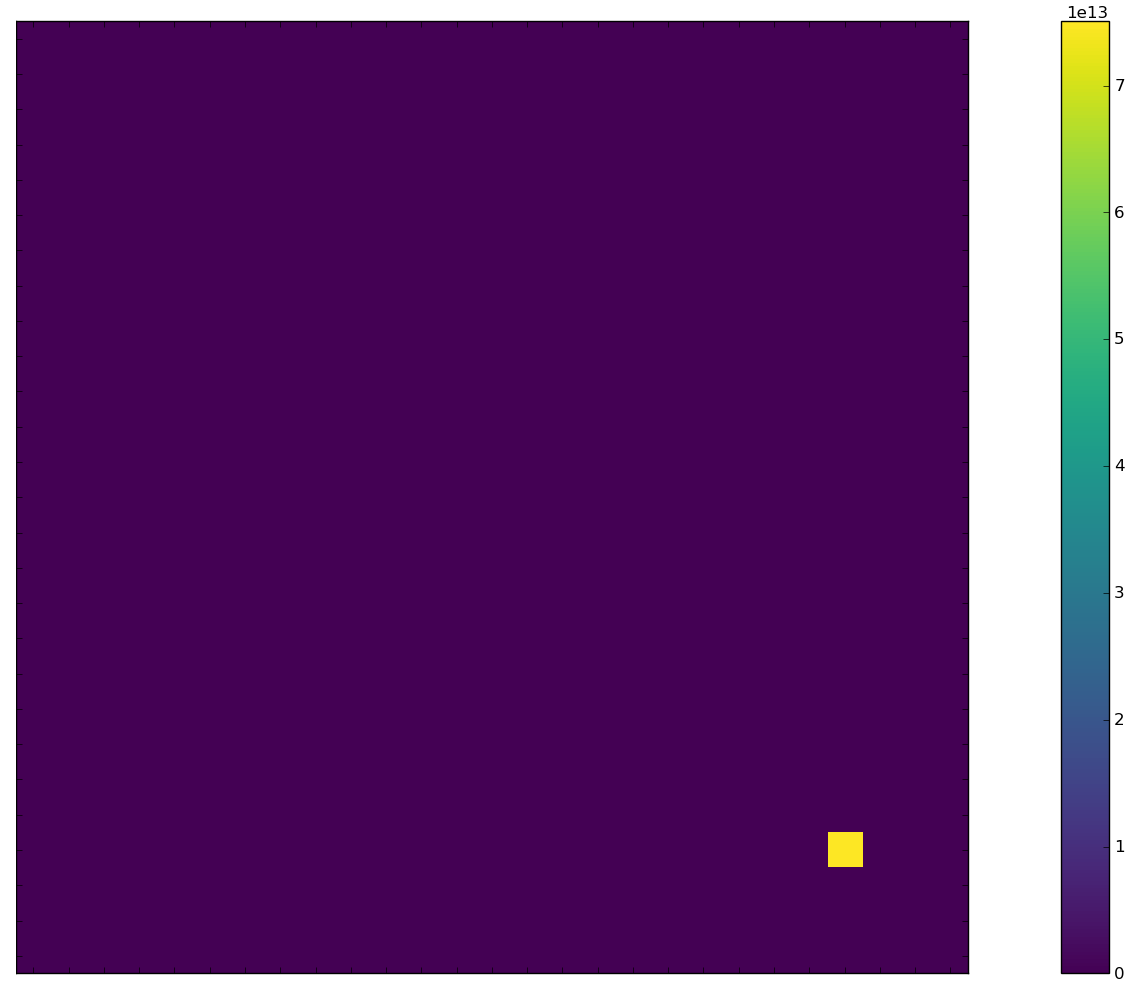
\includegraphics[width=\linewidth]{../figures/anotherfullheatmap.png}
	\caption{Correlation matrix of data with outliers (cellphone)}
   	\end{subfigure}
   	\begin{subfigure}[p]{0.4\linewidth}
    	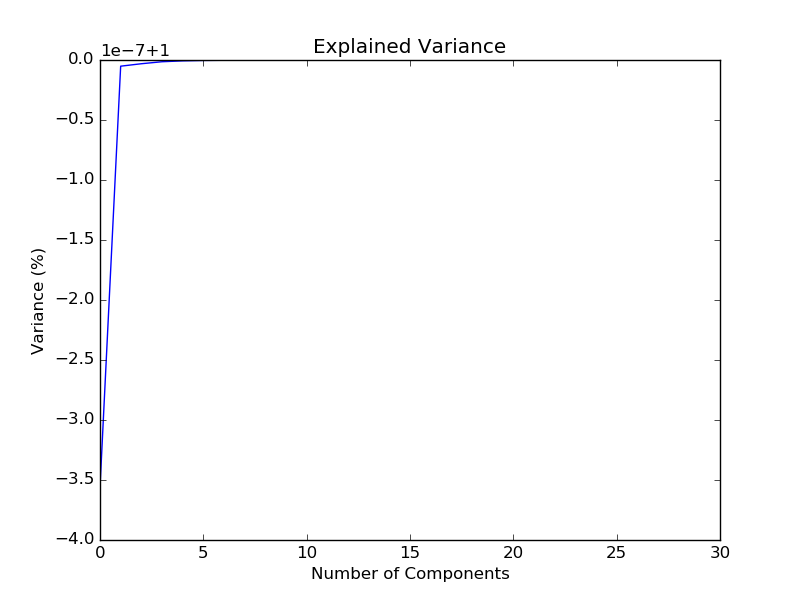
\includegraphics[width=\linewidth]{../figures/explained_variance.png}
	\caption{Variance elbow curve (cellphone)}
   	\end{subfigure}
\end{figure} 

We can see from the variance plot, and the correlation matrix above that a single feature column had variance so high that the relationship between all other features is obfuscated by such a large variance.  In addition, many of these columns have a variance of 0 (that is, all fields have the exact same value for the whole column) so they are useless when deriving some sort of insight for the data.  In most cases, they can ruin the results of a model.  So we needed to find a way to remove these useless columns and model-destroying outliers.

\newpage
So we had to experiment with several different methods of outlier removal in order to preprocess the data in such a way that the algorithms would work.  We used a modified z-score approach to remove rows with outliers that dominated the variance of their columns.  The standard z-score approach is to divide the difference of the column mean and the data value by the standard deviation of the column.  The modified z-score uses the difference between the median and the value, and divides by the mean absolute deviation instead.  This method is more robust to outliers, and helps us calculate them. After doing these two steps, we end up with a much better looking correlation matrix and elbow curve

\begin{figure}[!htbp]
  	\centering
   	\begin{subfigure}[p]{0.4\linewidth}
    	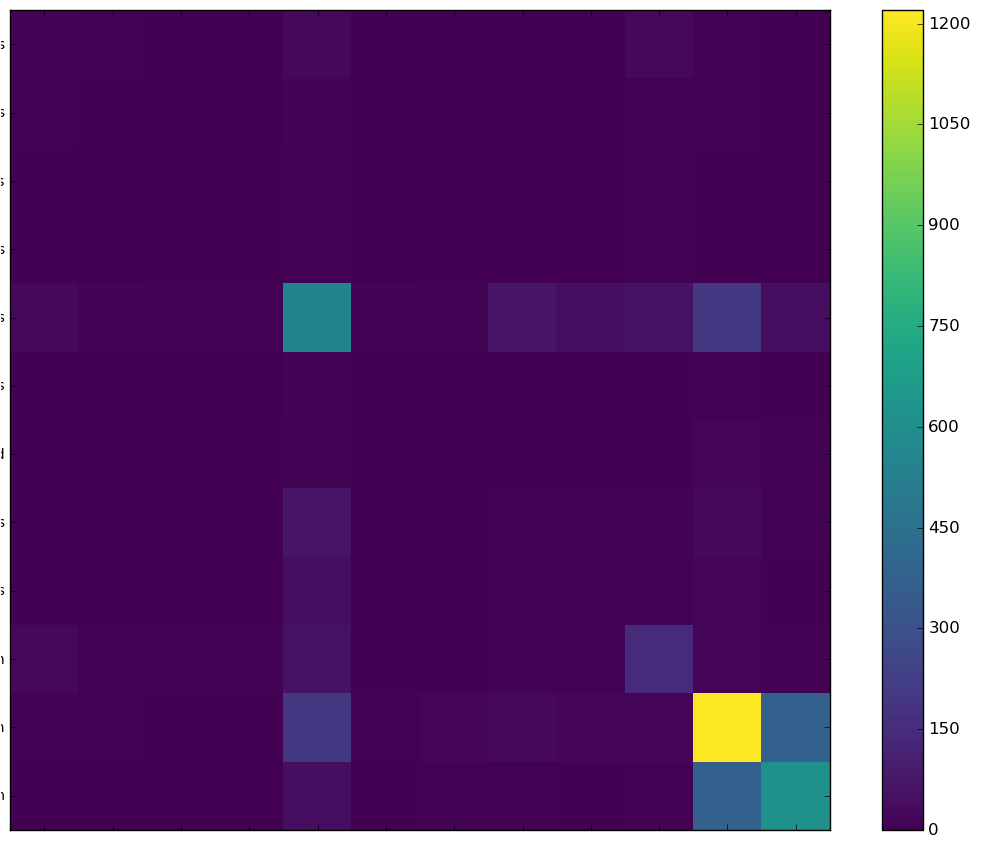
\includegraphics[width=\linewidth]{../figures/redo/cellphone/cp_covariance.png}
	\caption{post-processed correlation matrix (cellphone)}
   	\end{subfigure}
   	\begin{subfigure}[p]{0.4\linewidth}
    	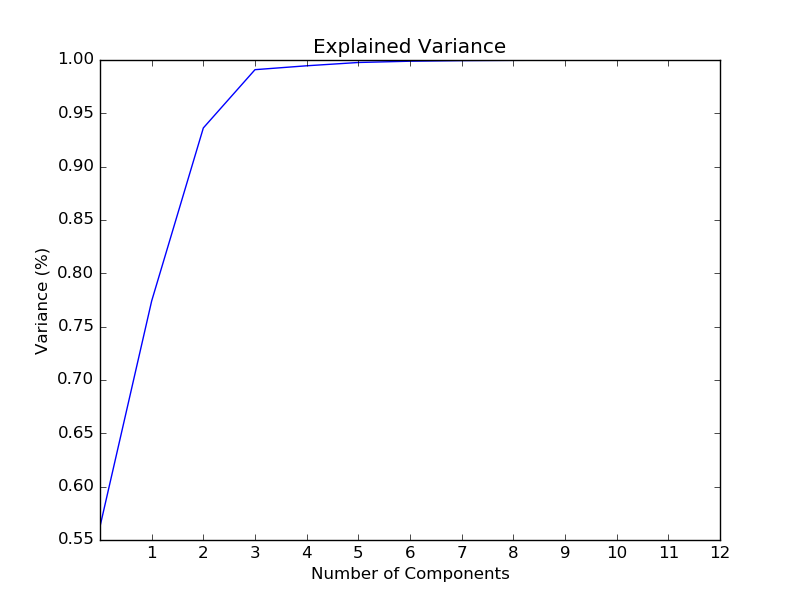
\includegraphics[width=\linewidth]{../figures/redo/cellphone/cp_explained_variance.png}
	\caption{Variance elbow curve (cellphone)}
   	\end{subfigure}
\end{figure} 

Keep in mind that the data we are looking at here is specifically the cellphone data.  The pre-processed correlation matrix shown below suffers from the same problems that the cellphone data did:

\begin{figure}[!htbp]
  	\centering
   	\begin{subfigure}[p]{0.4\linewidth}
    	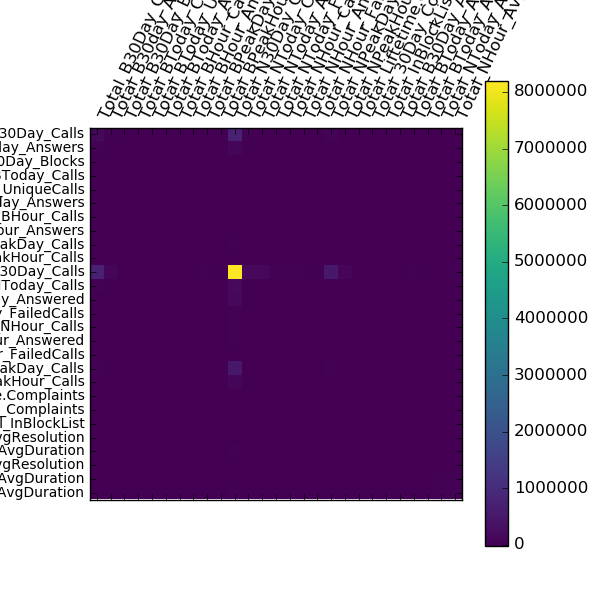
\includegraphics[width=\linewidth]{../figures/landline/raw_correlation_matrix.png}
	\caption{unprocessed correlation matrix (landline)}
   	\end{subfigure}
   	\begin{subfigure}[p]{0.4\linewidth}
    	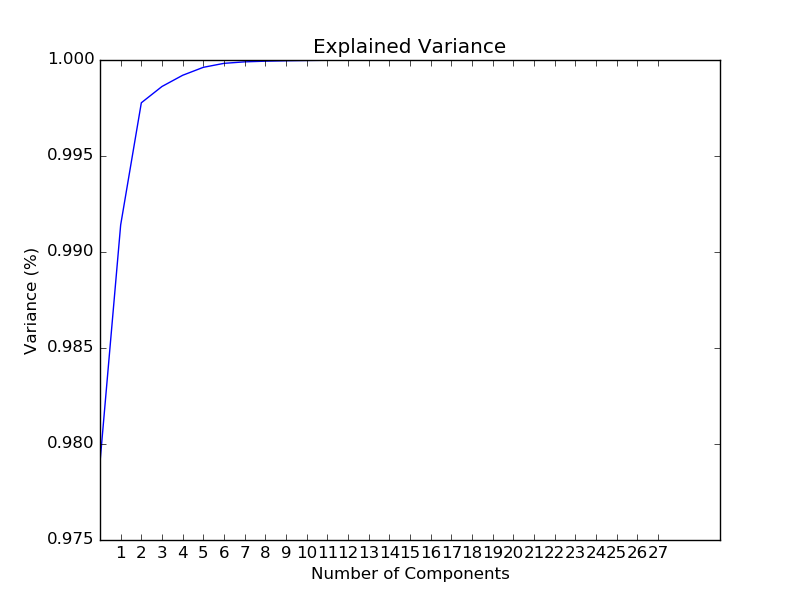
\includegraphics[width=\linewidth]{../figures/landline/raw_variance_curve.png}
	\caption{Variance elbow curve before preprocessing (landline)}
   	\end{subfigure}
\end{figure} 

\newpage
And after feature selection, and outlier detection and removal:

\begin{figure}[!htbp]
  	\centering
   	\begin{subfigure}[p]{0.4\linewidth}
    	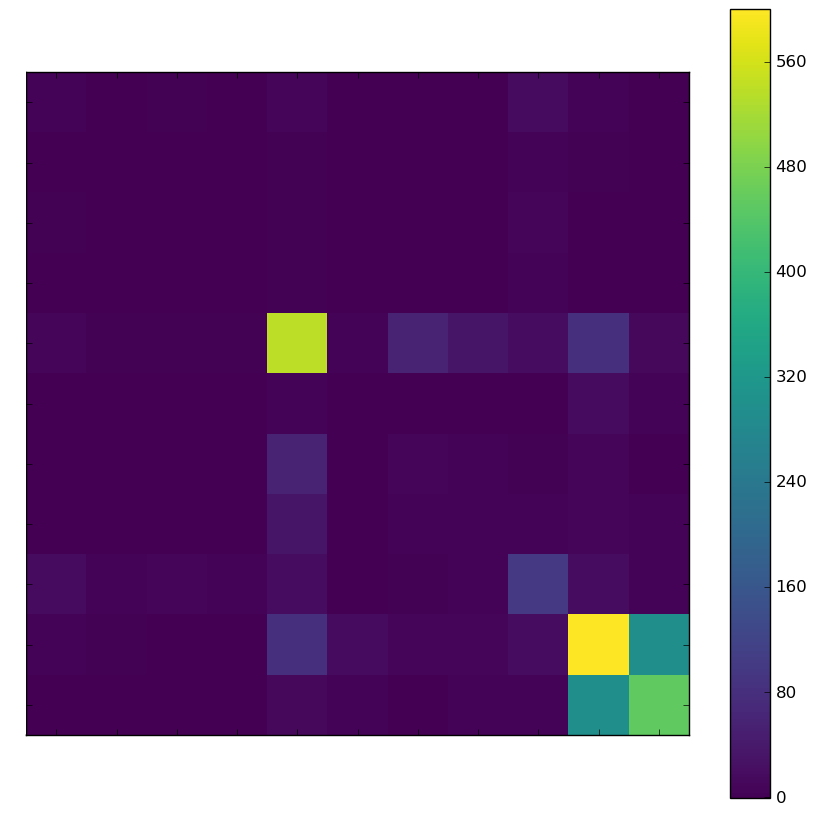
\includegraphics[width=\linewidth]{../figures/redo/landline/ll_covariance.png}
	\caption{post-processed correlation matrix (landline)}
   	\end{subfigure}
   	\begin{subfigure}[p]{0.4\linewidth}
    	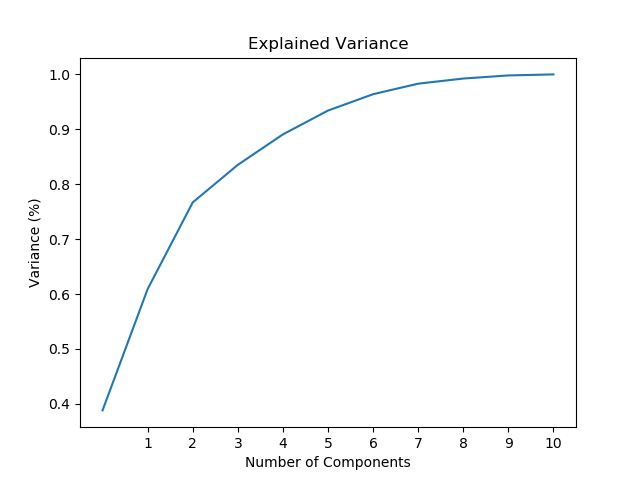
\includegraphics[width=\linewidth]{../figures/redo/landline/ll_explained_variance.png}
	\caption{Variance elbow curve (landline)}
   	\end{subfigure}
\end{figure} 

So what does this mean? Well the correlation matrix shows variables which vary together.  if you look at one of the pre-processed matrices, you can see that a single variable contains most of the variance for the entire dataset.  When a column and row is mostly purple, and one point is bright yellow, this means that the given variable there is highly independent from the other variables, and it contains much of the variance for the entire set.  As we can see post-processing, a few of the variables roughly vary together, with a few variables containing most of the variance of the dataset.

However, we want to find which variables are really responsible for the variance in the data.  If you observe the two \textit{explained variance} plots for each of the datasets, you can see that we get more than our minimum of 85\% of the data with only two principal components.  This is great because then we can plot the raw PCA output to a plot and study it there.  Sometimes, the number of principal components required for our 85\% threadhold for a given dataset can be 7, 8, or some higher dimensional number that we can't visualize.  So we have to perform PCA, then find some projection algorithm to bring the PCA data down to a dimension we can understand.  This can obscure the results and make interpretation more difficult.  Luckily we don't have that problem here...

\newpage
Which is actually where I went wrong. After much frustration, I found that there are multiple ways to perform PCA.  And the way that Python did it (using scikit-learn) computed PCA in a way which accumulated much of the variance in a few principal components, but tended to mash the points together such that separation is difficult to see.  Another way is using singular value deocmposition, which is supposedly the preferred method for numerical accuracy. Just as an example, here is the first method and the second, side by side, in R, using the first two principal components on our landline dataset:
\begin{figure}[!htbp]
  	\centering
   	\begin{subfigure}[p]{0.45\linewidth}
    	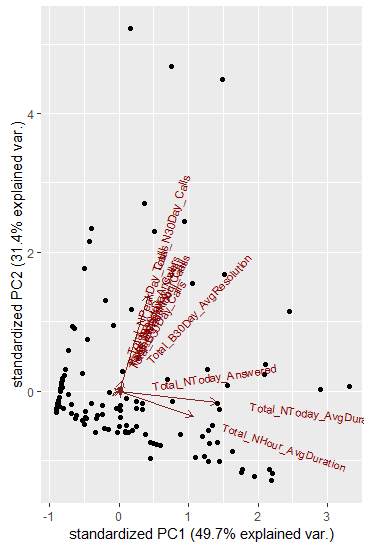
\includegraphics[width=\linewidth]{../figures/R/Rplot.png}
	\caption{sci-kit learn eigen-correlation method}
   	\end{subfigure}
   	\begin{subfigure}[p]{0.45\linewidth}
    	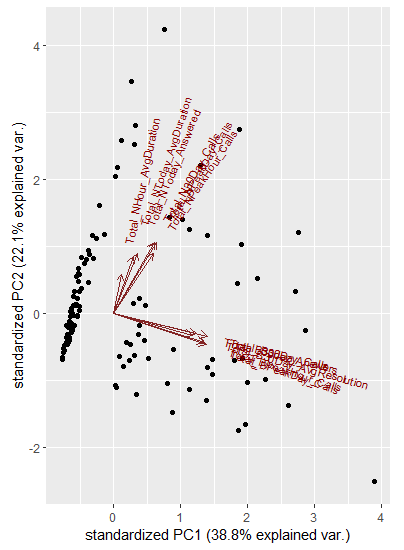
\includegraphics[width=\linewidth]{../figures/R/landline_removedoutliers.png}
	\caption{Singular Value Decomposition}
   	\end{subfigure}
\end{figure}

Notice how the left plot is exactly similar to the one from scikit-learn:
\begin{figure}[!htbp]
  	\centering
   	\begin{subfigure}[p]{0.55\linewidth}
    	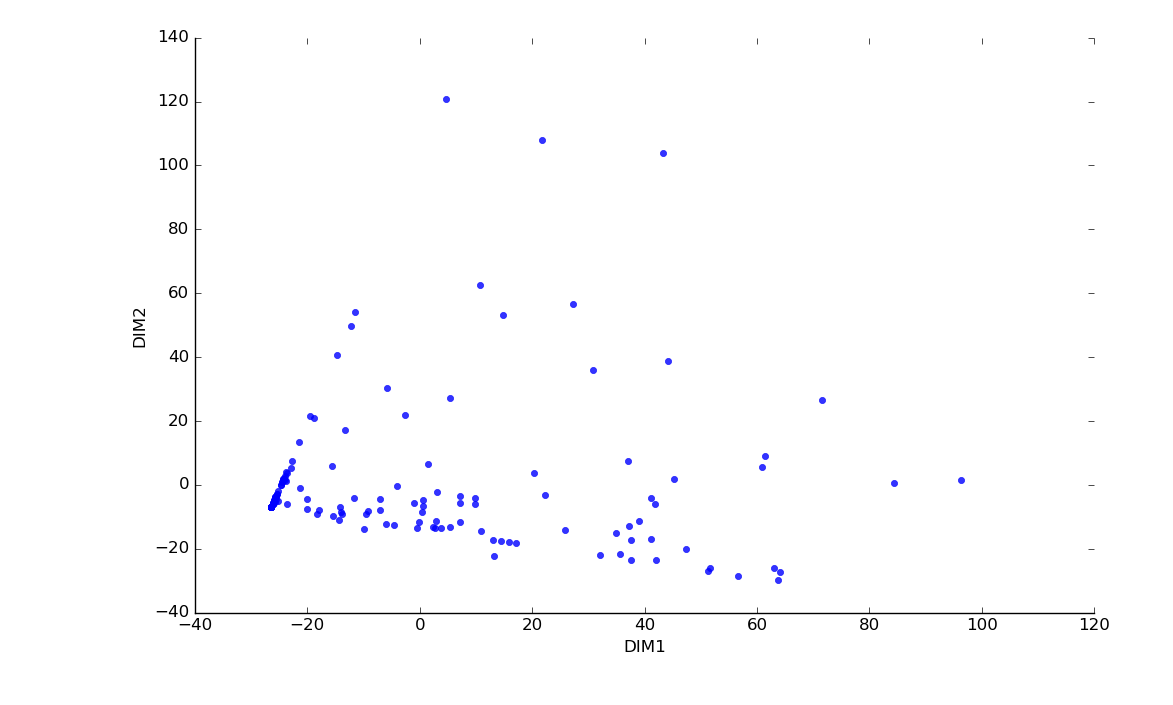
\includegraphics[width=\linewidth]{../figures/sklearnpca.png}
	\caption{post-processed correlation matrix (landline)}
   	\end{subfigure}
\end{figure} 

\newpage
Note the arrows on the previous graphs are features of the plot that help us understand what the principal components are comprised of.  However, this better separation comes with a caveat.  We can't achieve the 85\% variance with just 2 principal components.  Now we need 5 for the landline data, and 6 for the cellphone data. After doing some experimental clustering on the data, we needed a way to see it.  We used an algorithm call \textit{Uniform Manifold Approximation and Projection (UMAP)}.   The initial results look very promising, but there is a catch.  Projection algorithms can often disrupt the global structure of the data, so it isn't always safe to cluster on the output.  With that said, here are the initial outputs of the projections:

\begin{figure}[!htbp]
  	\centering
   	\begin{subfigure}[p]{0.4\linewidth}
    	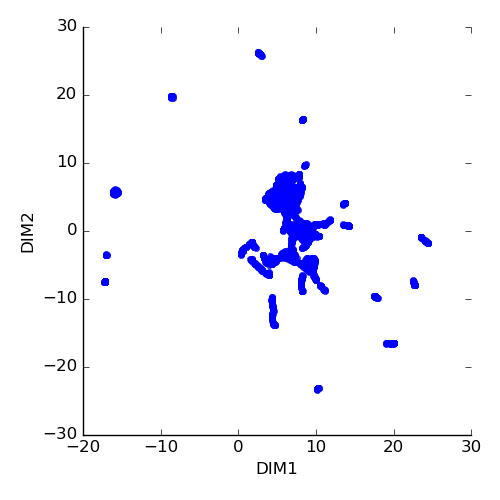
\includegraphics[width=\linewidth]{../figures/redo/cellphonemap.png}
	\caption{UMAP cellphone projected data}
   	\end{subfigure}
   	\begin{subfigure}[p]{0.4\linewidth}
    	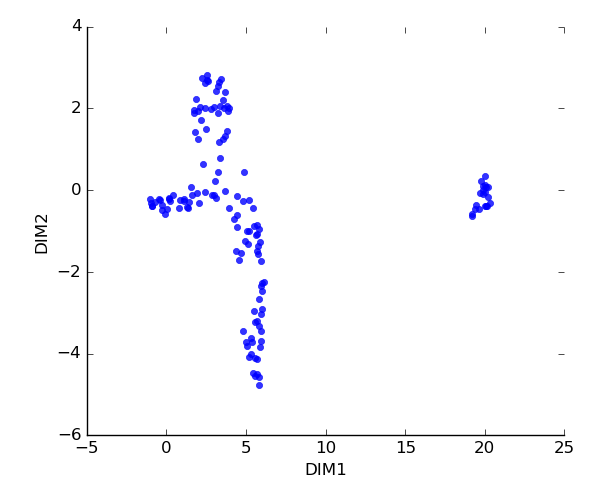
\includegraphics[width=\linewidth]{../figures/redo/landlinemap.png}
	\caption{UMAP landline projected data}
   	\end{subfigure}
\end{figure} 

One of the goto algorithms for clustering is KMeans. KMeans is an algorithm that seeks to partition the data into $k$ different groups where each data point belongs to the cluster whose mean it is closest to. With each point added, the mean of the cluster may shift a little, but it seeks to build samples based on distance to the mean of that sample.  To find the optimal value of $k$, that is, how many "samples" we have, we try a bunch of different values of $k$ and sum the distance from each point to its center:

\begin{figure}[!htbp]
  	\centering
   	\begin{subfigure}[p]{0.45\linewidth}
    	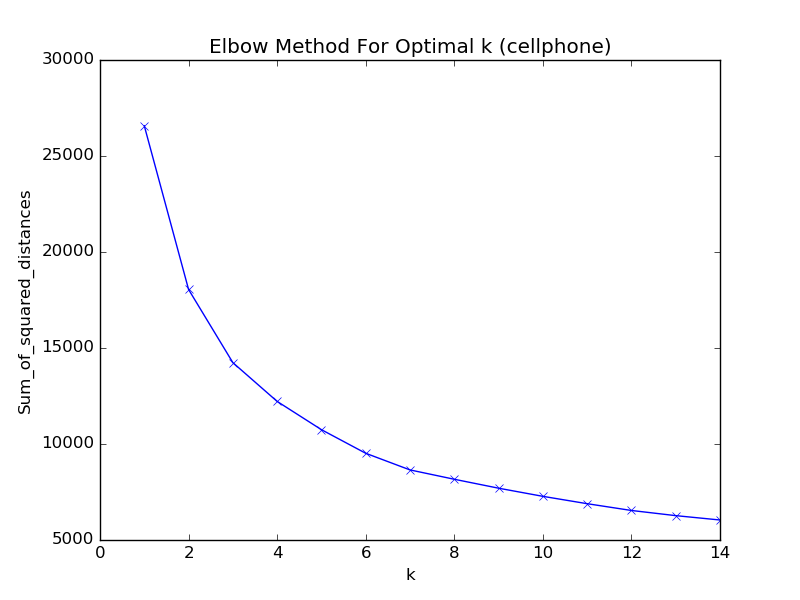
\includegraphics[width=\linewidth]{../figures/redo/cellphone/cp_optimal_k.png}
	\caption{Optimal $k$ for cellphone data}
   	\end{subfigure}
   	\begin{subfigure}[p]{0.45\linewidth}
    	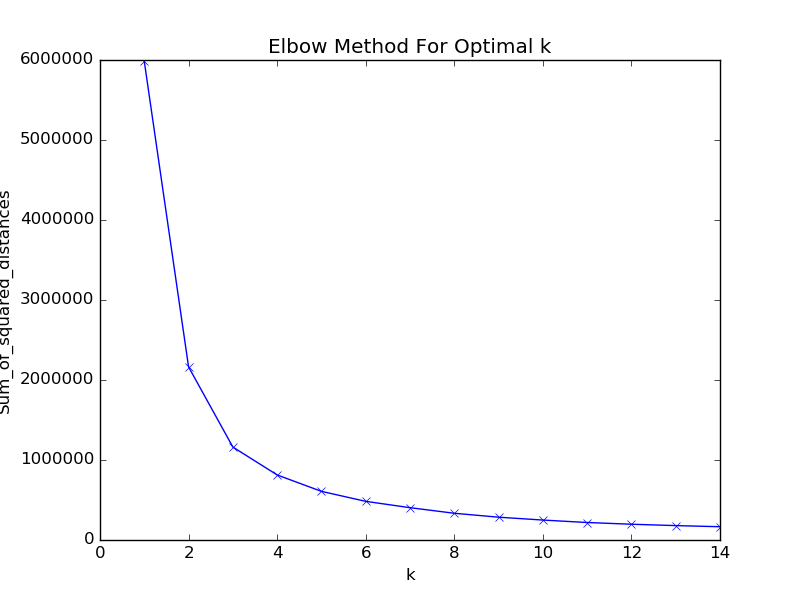
\includegraphics[width=\linewidth]{../figures/redo/landline/ll_optimal_k.png}
	\caption{Optimal $k$ for landline data}
   	\end{subfigure}
\end{figure} 

\newpage
I produced a few of the plots with different values of $k$ for the landline data, simply to show that you can't always trust the projection data:
\begin{figure}[!htbp]
  	\centering
   	\begin{subfigure}[p]{0.45\linewidth}
    	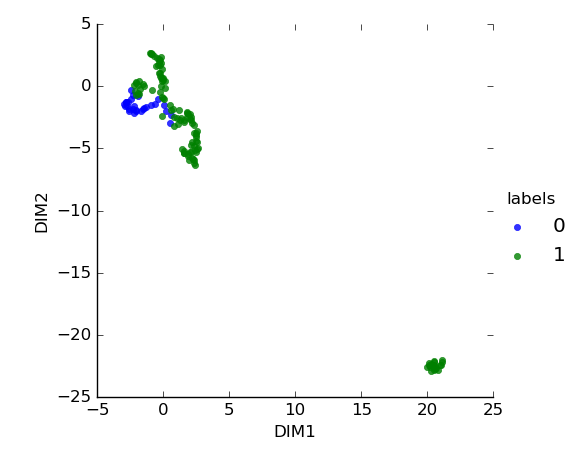
\includegraphics[width=\linewidth]{../figures/redo/landline/ll_kmeans2.png}
	\caption{$k=2$ for landline data}
   	\end{subfigure}
   	\begin{subfigure}[p]{0.45\linewidth}
    	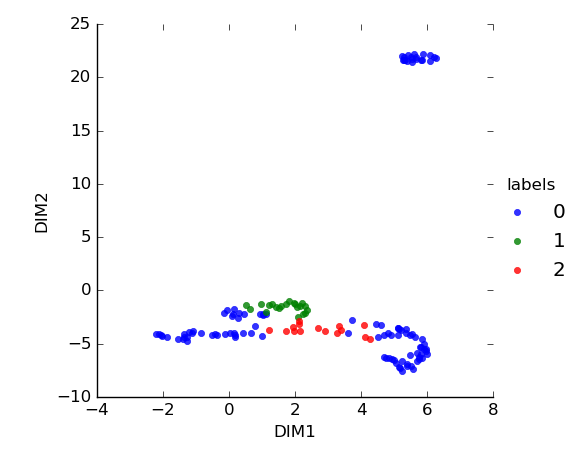
\includegraphics[width=\linewidth]{../figures/redo/landline/ll_kmeans3.png}
	\caption{$k=3$ for landline data}
   	\end{subfigure}
\end{figure} 
\begin{figure}[!htbp]
  	\centering
   	\begin{subfigure}[p]{0.45\linewidth}
    	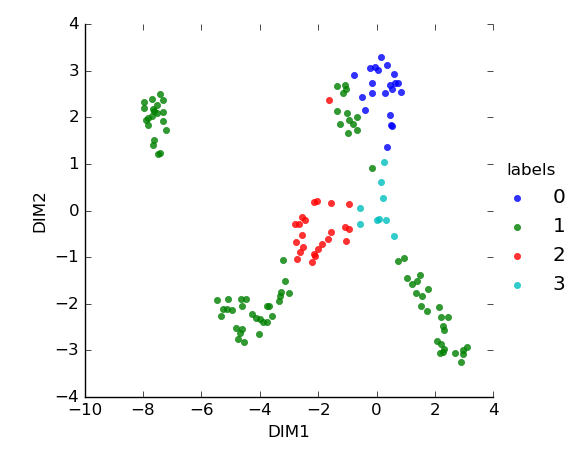
\includegraphics[width=\linewidth]{../figures/redo/landline/ll_kmeans4.png}
	\caption{$k=4$ for landline data}
   	\end{subfigure}
\end{figure} 

The first most glaring point is that the projection is different every time, and it depends on where the projection algorithm starts its seed.  There is consistently a large cluster separated from a small, dense cluster every time, which is interesting.  However, recall that a point belongs to the cluster whose mean it is closest too.  And since our optimal value of $k$ is actually 3 in regards to the landline data, then in it's hyper-dimensional space, the blue groups must be closer together than they are to the red or green, even if it looks like one blue piece is floating far away.  This sort of experimentation will continue with a variety of different algorithms, as well as hyper-parameters for those algorithms, to optimize the separation of the structure.  There is no one-size-fits all approach, and each algorithm answers the question in its own way.
\subsection{Risks}
\begin{itemize}
\item \textbf{False Positives:} We reduce this risk by first setting a threshold below which "normal" callers are placed.  By doing so, we reduce the amount of variance in the data and can focus entirely upon the anomalies.  Since we are only dealing with the anomalies, the average person won't be accidently detected, and as a consequence the different between a legitimate anomaly (a person with real needs to make many calls) and a spam caller will become more apparent, as the structure of the data overall won't be obscured by the average person.
\end{itemize}
\subsection{Tasks}
The tasks are administered ad-hoc.  Since data science is highly experimental, team members often worked on the same problem from different approaches, and there was discussion and agreement on which result to accept.
\begin{itemize}
\item Split data into cellphone and landline partitions
\item Map and Reduce calls from streaming data
\item Speak with company and decide on anomaly boundary
\item Outlier Detection
\subitem log-transform
\subitem modified z-score
\item Principal Component Analysis
\subitem find important features
\item Clustering
\subitem KMeans
\subitem Gaussian Mixture Model
\subitem Experiment with hyperparameters to optimize results
\item discuss results with First Orion
\end{itemize}
\newpage
\subsection{Schedule}
The schedule was flexible the entire project and team members helped when they could.  Communication between the team and First Orion was difficult, and I feel as though the management dumped our team onto their data science team.  The data science team seemed unprepared to mentor college students (not their fault), especially since it was only a single person who also had a job to do on their own
\begin{enumerate}
\item Split Data into cellphone and landline partitions | \textit{Mid-January} | Damian, Liam
\item Map and Reduce calls from streaming data | \textit{Mid-January} | Damian, Liam
\item Speak with company and decide on anomaly boundary | \textit{End of January} | Liam
\item Outlier Detection | \textit{Mid-February} | Liam
\subitem log-transform | \textit{Mid-February} | Spencer
\subitem modified z-score | \textit{Mid-February} | Jonah
\item Principal Component Analysis | \textit{End of February} | All
\subitem find important features | \textit{End of February} | All
\item Clustering | \textit{Ongoing} | All 
\subitem KMeans | Liam, Damian
\subitem Gaussian Mixture Model | Spencer, Jonah
\subitem Experiment with hyperparameters to optimize results | All
\item Discuss results with First Orion | \textit{Ongoing} | All
\end{enumerate}
The purpose of listing some tasks as ongoing, is because this project is a focus of my career, and I want to personally see the end of the project, and what First Orion does with the results We've produced.  At this point the project is more volunteer work or some ad-hoc internship, and not about school
\subsection{Deliverables}
\begin{itemize}
\item \textbf{R code:} This is the code use to wrangle some of the data and split it into subsets, as well as detect and remove outliers
\item \textbf{Python code:} This is the code used to run clustering and plotting algorithms on, produce plots, etc.
\item \textbf{Insights:} Our project won't neccesarily have a deliverable, the deliverable is, the insights we can provide with our techniques, that is differentiating between high-volume legitimate callers and spam callers. For example, separate the mobile/landline numbers into meaningful clusters and analyze the features to discover which ones are discriminatory. Also, the spam callers will have to be investigated on their own to verify that they are spam
\end{itemize}

\section{Key Personnel} 
\begin{itemize}
\item \textbf{Liam Dillingham} - A senior Computer Science and Mathematics (Statistics) double major in the CSCE and FullBright college at University of Arkansas.  Complete relevant courses: STAT 4003 (Statistical Methods), Machine Learning (CSCE 5063), Big Data Analytics and Management (CSCE 5273), and Computational Statistics (STAT 5443).  Relevant experience comes from previous internships as a dual-role software engineer/data scientist, as well as course-related projects.  Tasks included working with industry champions to produce satisfactory results and develop code and insights from data

\item \textbf{Industry Champion: Nysia George} - Nysia is a senior level data scientist at First Orion, and was tasked to be our mentor during the course of the project.  She is who we brought our results to, asked questions, and took guidance in order to provide her with results that aided in her work and improving the company's products.
\end{itemize}

\section{Facilities and Equipment}
Initially we believed we needed a larger computer in order to run some of the more complex algorithms on the data, however, after sufficient preprocessing, we were able to reduce the size and complexity of the data to a much more manageable scale.

\end{document}


































